\documentclass[review]{elsarticle}
\usepackage{lineno,hyperref}
\modulolinenumbers[5]
\usepackage{dcolumn, graphics, graphicx, grffile, amsmath, amsthm, amssymb, color, colortbl}
\usepackage{subfig}
\usepackage{enumitem}
\usepackage{booktabs}
\usepackage{float}
\usepackage{geometry}
\geometry{verbose,tmargin=2.5cm,bmargin=2.5cm,lmargin=2.5cm,rmargin=2.5cm}
%\usepackage{authblk}
\usepackage[latin1]{inputenc}
\usepackage{tikz}
\usetikzlibrary{shapes,arrows}
\usepackage{verbatim}
\usepackage{setspace}
\usepackage{array}
\usepackage{multirow}
\usepackage{blkarray}
\usepackage{mathtools}
\usepackage{natbib}
% boldface lowercase letters for vectors
\newcommand{\xbf}{\ensuremath{\mathbf x}}

\journal{Spatial Statistics}
\bibliographystyle{model2-names.bst}\biboptions{authoryear}

\begin{document}
\begin{frontmatter}

\title{Grid-spacing and the quality of abundance maps for species that show spatial autocorrelation and zero-inflation}

%% Group authors per affiliation:
\author[1]{Olga Lyashevska}
\ead{olga@herenstraat.nl}

\author[2]{Dick J. Brus}
\ead{Dick.Brus@wur.nl}

\author[1]{Jaap van der Meer\corref{cor1}}
\ead{Jaap.van.der.Meer@nioz.nl}

\cortext[cor1]{Corresponding author}

\address[1]{Department of Marine Ecology\\
NIOZ Royal Netherlands Institute for Sea Research\\
P.O. Box 59 1790 AB Den Burg\\
Texel, The Netherlands}

\address[2]{Alterra, Wageningen University and Research Centre\\
P.O. Box 47, 6700AA\\
Wageningen, The Netherlands}

\begin{abstract}
The effect of grid-spacing on the quality of species abundance maps is explored for species that show zero-inflation and spatial autocorrelation.
Species abundance maps constructed through a generalised linear geostatistical modelling approach were subsampled by grid-sampling with 200, 400, 800, 1600, 3200, and 6400 m grid-spacing.
The model parameters at 1000 validation locations were predicted by simple kriging with an external drift, using silt, silt squared and altitude as external drift variables. 
Two approaches were used for choosing kriging model parameters: fixed parent-model parameters and variable sample-specific parameters, giving a rough estimate of the sampling distribution.
A total of 100 grid-samples was obtained using the first approach and 4 grid-samples using the second approach. 
Both approaches showed an increase in the Mean Squared Error with increasing spacing.
This increase, however,  was not smooth in the second approach but showed a steep rise at 3200 m when the number of sampling locations decreased from about 400 to about 200.
We therefore recommend to have at least 400 sampling locations.
\end{abstract}

\begin{keyword}
count data, generalized linear geostatistical modeling, autocorrelation, zero-inflation, grid-spacing
\end{keyword}

\end{frontmatter}

\linenumbers

\section{Introduction}

The relationship between species and their environment is generally described by species distribution models, also known as habitat suitability or environmental niche models \citep{guisan2005}. Such models are constructed using survey data available at a limited set of sampling locations and allow one to create predictive species distribution maps on the basis of environmental data which are usually available at a much larger set of locations \citep{guisan2000}. The number of sampling locations is known to affect the accuracy of the species distribution models and maps \citep{stockwell2002, wisz2008}.  Knowledge of the trade-off function between the number of sampling locations and the accuracy of the predictions is usually not obtained a priori  with the risk that the survey either does not provide the required accuracy or is unnecessarily costly \citep{caughlan2001,reynolds2011}.

Yet, the effect of sample size on the accuracy of species distribution models was evaluated by few \citep[see e.g.][]{stockwell2002,pearson2007,wisz2008,hanberry2012}. For example, \citet{stockwell2002} assessed sample size requirements for modelling bird species in Mexico by random sampling 1 to 100 locations. \citet{wisz2008} considered three sample sizes (10, 30, and 100 locations) to evaluate the quality of model predictions using data for 46 species obtained from natural history collections. Finally, \citet{hanberry2012} used sample sizes ranging from 30 to 2500 locations to model tree species in northeasten  Minnesota. All these studies consider presence--absence maps, but often, predictive species abundance maps in the form of numerical or biomass density are to be preferred,  because they are more informative than presence--absence maps \citep{vieira2012, cozzi2013}.  \citet{fortin1989} constructed such maps using sugar-maple tree density data gathered in  southwestern Qu\'{e}bec.  The authors evaluated the ability to predict spatial patterns using different sample sizes and designs. They considered two sample sizes of 50 and 64 points, both derived from a 200-point dataset.

Using real datasets only, as \citet{fortin1989} did, the possibilities of studying the effect of the type of sampling design and sample size are limited. This limitation was recognised in recent studies, such as those  by \citet{perner2004, rachowicz2006, bijleveld2012} and \citet{foster2014}. These studies follow an approach whereby first a spatial field resembling reality as much as possible, a peseudo-reality, is simulated, which is subsequently sampled using different sampling designs. The performance of sampling designs is then compared by confronting predictions with simulated values that serve as ground-truth.  \citet{zurell2010} call this the virtual ecologist approach.  Following this approach, \citet{bijleveld2012}, for example, used the results of an existing intertidal benthic monitoring programme to construct various spatial models with an exponential spatial autocorrelation function. With these models they simulated virtual populations with a Normal distribution and sampled these populations using different sampling designs. They provided a trade-off function between sampling distance and prediction error which was rather flat for those virtual species that hardly showed spatial autocorrelation, but much steeper for species with strong spatial autocorrelation. The authors assumed normality of the data which was clearly violated by the empirical data if only because of the many zero observations.

The assumption of normality is a common practice, but when we are dealing with species abundance (count) data, even the more obvious Poisson distribution is rarely applicable. Ecological count data have two properties that ask for a specific treatment, other than relying on the classical assumption of independent and normally distributed data. These properties are zero-inflation \citep{martin2005, clarke1988, lewis2011} and spatial autocorrelation, i.e. nearby observations are more similar than observations far apart, even when environmental conditions do not differ. Hitherto most studies have dealt with these two properties, but only one at a time \citep{tyre2003, bijleveld2012}.

For example, the first property was accounted by \citet{tyre2003} who considered the zero-inflated negative binomial model, but ignored autocorrelation. Ignoring spatial autocorrelation in simulation studies on how sampling designs affect the accuracy of estimates of population- or model parameters or the accuracy of spatial predictions, may lead to biased estimates of this accuracy \citep{legendre2002}.

Contrary to \citet{tyre2003}, the \citeauthor{bijleveld2012} study took account of the autocorrelation by using a stochastic model that included spatial autocorrelation of the error. But, as we mentioned earlier, they simulated normally distributed data. Clearly, there is a need to integrate both properties in a single study and to examine how zero-inflation and autocorrelation may affect recommendations concerning the optimal sampling design, sample size, and distance between samples.

Only few studies simultaneously address zero-inflation and autocorrelation for species abundances \citep[see e.g.][]{recta2012, boyd2015}, but none of them address the question of optimal sampling design.  We fill this gap by following a paper by \citet{lyashevska2015a} in simulating fields with zero-inflated, spatially autocorrelated count data, and sampling the fields repeatedly with different sampling designs. More specifically, we will sample the fields by grid-sampling with a varying spacing. The objective of this paper is to quantify the trade-off between the grid-spacing and the accuracy of predictions of species-abundance model-parameters on a fine grid for mapping, for species that show zero-inflation and spatial autocorrelation. Most species will show these two properties.

\section{Materials and methods} \label{sec:methods}

%We provide a brief description of the statistical methodology of modelling zero-inflated, auto-correlated species abundance data. For more details we refer to the companion paper \citep{lyashevska2015}.

\subsection{Data}

Data used in this paper were zero-inflated (66\% are zeros) and autocorrelated counts of a benthic species \textit{Macoma balthica} (Fig.~\ref{fig:AbundanceRaw}) that were collected in the yearly Synoptic Intertidal Benthic Surveys (SIBES) monitoring programme conducted in the Dutch Wadden Sea \citep{bijleveld2012, compton2013}. The study area, bordered by the barrier islands on the north and by the mainland coast on the south, is formed by intertidal and subtidal mudflats and gullies. The monitoring network consists of 3451 permanent locations on intertidal mudflats at the nodes of a 500 m grid. The square grid is supplemented by 578 locations. These locations were selected by first selecting 578 out of the 3451 grid-points by simple random sampling without replacement. Then at each selected grid-point one point was selected at a uniformly distributed distance between 0 and 250 m distance from the grid-point, in a direction randomly chosen from the four directions defined by the grid-lines \citep{bijleveld2012}.

The most important determinants of habitat structure used for mapping the abundance were sediment texture characteristic, more specifically the mass fraction of silt, and altitude (Amsterdam Ordnance Datum, Rijkswaterstaat \footnote{www.rijkswaterstaat.nl}). To be used as a predictor in mapping, the covariate must be known everywhere in the study area. Therefore the mass fraction of silt was interpolated by inverse distance weighting in ArcGIS 10.0. 

\subsection{Overview of evaluation method}
The starting point of the our procedure for evaluating the sampling designs is a model for the spatial distribution of the zero-inflated and autocorrelated count data. This spatial distribution is modelled through a spatial zero-inflated Poisson mixture model(ZIP)\citep{lambert1992, agarwal2002}:
\begin{equation}
    P(Y_i=y)=
\begin{cases}
\pi_i+(1-\pi_i)\text{exp}(-\mu_i) & y=0 \\
(1-\pi_i)\frac{\text{exp}(-\mu_i)\mu_i^{y}}{y!}& y=1,2,3,\ldots
\end{cases}
\end{equation}
where $Y_i$ is the count at location $i$, $\pi_i$ the probability of a Bernoulli zero at location $i$, and $1-\pi_i$ is the probability of a Poisson count, either zero or non-zero. The intensity (mean number of individuals) of the Poisson process at location $i$ is $\mu_i$. The first part of the model is the overall probability of zero \citep{hilbe2007}.

The parameters $\pi_i$ and $\mu_i$ at location $i$ are random variables modelled by the following submodels:
\begin{eqnarray} \label{eq:glsm}
\text{logit}(\pi_{i})=\text{log}(\frac{\pi_{i}}{1-\pi_{i}})=\xbf_{\mathrm{B},i}^{T}\boldsymbol{\beta}_{\rm{B}} + \eta_{\mathrm{B},i} \nonumber \\
\text{log}(\mu_i)=\xbf_{\mathrm{P},i}^{T}\boldsymbol{\beta}_{\rm{P}} + \eta_{\mathrm{P},i}
\end{eqnarray}
with $\xbf_{\mathrm{B},i}$ and $\xbf_{\mathrm{P},i}$ vectors with covariates at location $i$, $\boldsymbol{\beta}_{\mathrm{B}}$ and $\boldsymbol{\beta}_{\mathrm{P}}$ vectors with regression coefficients, and $\eta_{\mathrm{B},i}$, $\eta_{\mathrm{P},i}$ residuals of the spatial trend. Note that the model parameters can be modelled by different sets of covariates.

The residuals $\eta_{\mathrm{B},i}$, $\eta_{\mathrm{P},i}$ at any location $i$ are random variables. The probability distribution of the residuals at all locations in the study area was modelled as
\begin{eqnarray}
\left[
\begin{array}{c}
\boldsymbol{\eta}_{\mathrm{B}} \\
\boldsymbol{\eta}_{\mathrm{P}} \\
\end{array}
\right]&\sim& \mathcal{N}\left(
\left[
\begin{array}{c}
\mathbf{0} \\
\mathbf{0} \\
\end{array}
\right],
\left[
\begin{array}{cc}
\mathbf{C}_{\mathrm{B}} & \mathbf{0} \\
\mathbf{0} & \mathbf{C}_{\mathrm{P}} \\
\end{array}
\right]
\right)
\end{eqnarray}
with $\mathbf{C}_{\mathrm{B}}$ and $\mathbf{C}_{\mathrm{P}}$ covariance matrices. So note that we assumed that the Bernoulli and Poisson residuals were independent. For both random residuals we further assumed isotropy, so that the covariance of the residuals at any two locations was modelled as a function of the distance $h$ between the two locations. For instance, for the Bernoulli residuals, the covariance was modelled as
\begin{equation}
    C_{\mathrm{B}}(h)=\sigma_{\mathrm{B}}^{2}\rho_{\mathrm{B}}(h; \phi_{\mathrm{B}})+\tau_{\mathrm{B}}^{2} \label{Ch}
\end{equation}
with $\sigma_{\mathrm{B}}^{2}$ the partial sill, $\phi_{\mathrm{B}}$ the range (distance parameter), $\tau_{\mathrm{B}}^{2}$ the nugget, and $\rho_{\mathrm{B}}$ the correlation function, for instance exponential or spherical \citep{webster2007}.

The two submodels in ~\ref{eq:glsm} are generalised linear mixed models, as they are the sum of a linear combination of covariates describing a spatial trend (fixed effect) and a spatially autocorrelated residual (random effect). \citet{diggle2007} names this type of models as generalised linear \textit{geostatistical} models.

Following \citet{diggle2007}, hereafter the sum of the trend and residual, representing the transformed model parameter, is referred to as the signal $S$, for instance $S_{\mathrm{B},i}= \mathbf{x}_{\mathrm{B},i}^{T}\boldsymbol{\beta}_{\rm{B}} + \eta_{\mathrm{B},i}$. For convenience, all the parameters in one model, including the type of correlation function, are collected in  a vector: $\boldsymbol{\theta}_{\mathrm{B}}=(\boldsymbol{\beta}_{\mathrm{B}}, \phi_{\mathrm{B}}, \tau_{\mathrm{B}}^2, \sigma_{\mathrm{B}}^2, \rho_{\mathrm{B}})$ and $\boldsymbol{\theta}_{\mathrm{P}}=(\boldsymbol{\beta}_{\mathrm{P}}, \phi_{\mathrm{P}}, \tau_{\mathrm{P}}^2, \sigma_{\mathrm{P}}^2, \rho_{\mathrm{P}})$.

The aim of the sampling strategy to be evaluated is to map the prevalence parameter $\pi$ of the Bernoulli distribution and the intensity parameter $\mu$ of the Poisson distribution. So note that the aim is not to predict the species abundance counts, but the \emph{expected} counts, conditional on covariates that define a spatial trend and the observed counts at the sample to be evaluated. We believe that predicting the counts themselves is not feasible in our situation, and besides not of practical relevance. 

Broadly speaking, our evaluation procedure is as follows. The SIBES data are used to calibrate a ZIP model. Several steps are involved in calibration. First, a ZIP model is fitted by maximum likelihood assuming that both residuals $\eta_{\mathrm{B},i}$ and $\eta_{\mathrm{P},i}$ are spatially independent. The fitted model parameters are then used to classify a zero count either as a Bernoulli or a Poisson zero, and to construct two datasets: the Bernoulli dataset with zeros (absent) and ones (present), and the Poisson subset, containing the SIBES locations with a one in the Bernoulli dataset, with counts. In the next step these two data sets are used to fit the two submodels for the parameters $\pi_i$ and $\mu_i$, but now accounting for spatial autocorrelation. This is done by simulating a large sample of signals $S_{\mathrm{B}}$ and $S_{\mathrm{P}}$ at the SIBES locations by Markov chain Monte Carlo (MCMC) using initial estimates of the model parameters, followed by Monte Carlo Maximum Likelihood (MCML) estimation of the model parameters.

The fitted model parameters are then used to predict the Bernoulli signal ($S_{\mathrm{B}}$) and Poisson signal ($S_{\mathrm{P}}$) at the nodes of a very fine square grid with a spacing of 100 m covering the study area. This prediction grid is extended with 1000 randomly selected validation locations in between the grid-points. The prediction method is simple kriging with an external drift, using silt, the squared values of silt, and altitude as external drift variables (predictors).

In the next step the predicted signals at the grid-nodes and validation points are used to simulate fields with count data. One field with statistics closest to those of the SIBES data is selected, and repeatedly sampled by grid-sampling. A range of grid-spacings is applied. Each selected grid is used to predict the model parameters $\pi_i$ and $\mu_i$ at the validation locations. By comparing these predictions with the true model parameters at the validation points the quality of the predictions is assessed. More details on all steps but the first two (calibration of ZIP model and prediction of signals) are given below. For details on the first two steps we refer to \citet{lyashevska2015a}.

\begin{enumerate}
\item
After prediction of the signal $S_{\mathrm{B}}$ at the nodes of the 100 m grid, 100 fields (square grids with spacing of 100 m) with spatially unstructured noise (white noise) are simulated from a Normal distribution with a variance equal to $\hat{\tau}^2_{\mathrm{B}}$. The predicted signal ($S_{\mathrm{B}}$) is added to the simulated fields with white noise. The resulting fields are backtransformed by second-order Taylor expansion to give 100 simulated fields of the prevalence parameter $\pi$ of the Bernoulli distribution. The same procedure is followed for the $S_{\mathrm{P}}$ to give 100 simulated fields of the intensity parameter $\mu$ of the Poisson distribution.

\item
Each simulated field of $\pi$ is used to simulate one field with presence/absence indicators, giving 100 fields with indicators. Besides, each simulated field of $\mu$ is used to simulate one field with Poisson counts, giving 100 fields with counts. These two sets of 100 fields are multiplied pair-by-pair, to give 100 fields with zero-inflated counts.

\item
From the 100 fields with zero-inflated counts, one field is selected with summary statistics closest to these summary statistics of the SIBES data. We used as summary statistics the fraction of zeroes, the mean of the Poisson counts, and the variance of the Poisson counts. This leads to three difference values per field. These differences values were standardized by dividing through their standard deviation. The weighted sum of the standardized differences was used as a selection criterion, with weights equal to 0.5 (for fraction of zeroes), 0.25 and 0.25. Apart from the field with zero-inflated counts, the two underlying fields with simulated prevalence parameter values $\pi$ and simulated intensity parameter values $\mu$ are selected, as these are needed in the validation (remind that the aim was to predict the model parameters $\pi$ and $\mu$). Fig.~\ref{fig:rawfield} shows a map of the product of $\pi$ and $\mu$, representing the unconditional intensity (unconditional expected count), and a map of the SIBES count data. There is a clear resemblance between the two maps.

\begin{figure}[htbp]
\subfloat[]{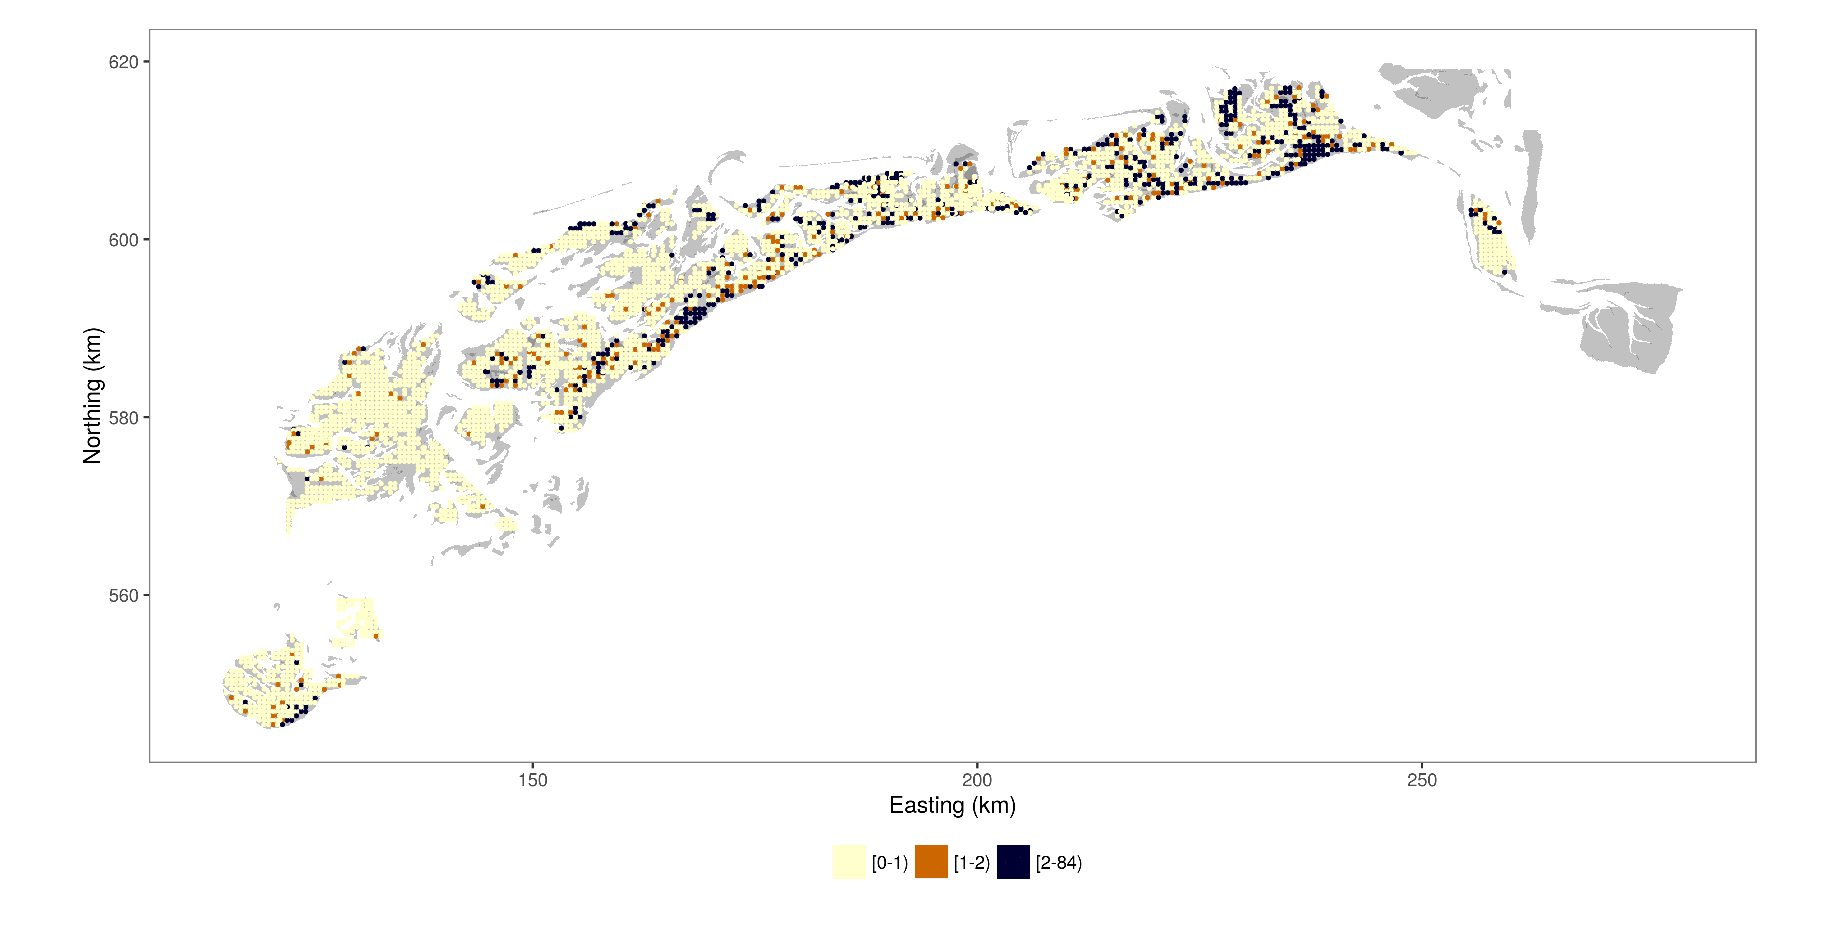
\includegraphics[width=0.9\linewidth]{AbundanceRaw} \label{fig:AbundanceRaw} }\quad
\subfloat[]{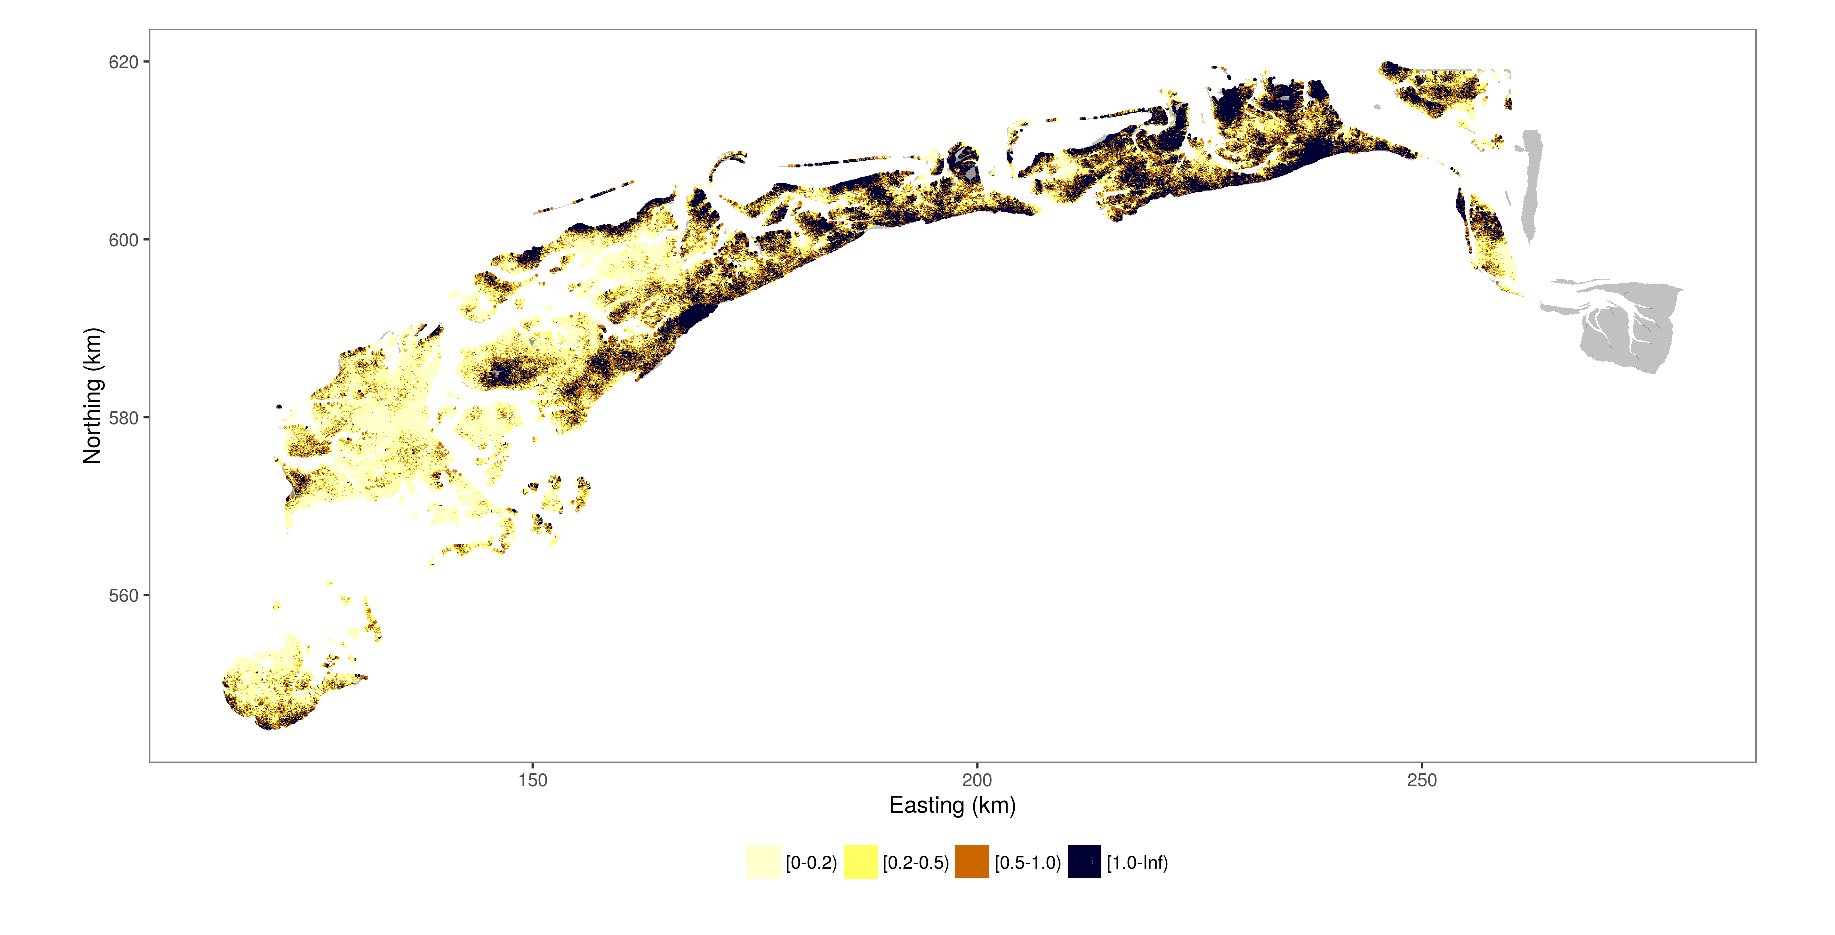
\includegraphics[width=0.9\linewidth]{pred.pimu.eps} \label{fig:field38} }
\caption{Empirical species abundance map of \textit{Macoma balthica} \protect\subref{fig:AbundanceRaw} and unconditional intensity map \protect\subref{fig:field38} predicted to the nodes of 100 m grid by simple kriging with an external drift. From \citet{lyashevska2015a}.}
\label{fig:rawfield}
\end{figure}

\item
The selected field with zero-inflated counts is sampled on a grid with a spacing of 200, 400, 800, 1600, 3200, and 6400 m. For each grid-spacing 100 samples are randomly selected. The corresponding number of grid-points was on average 28505, 7130, 1783, 446, 110, and 27, respectively. An overlay is made of the selected grids and the selected field with simulated zero-inflated counts to obtain the `pseudo-observations' of counts that will be used in prediction of the prevalence parameter $\pi$ and the intensity parameter $\mu$ at the validation locations.

\item
The model parameters $\pi$ and $\mu$ at the 1000 validation locations are predicted by the same method as used in simulating our pseudo-reality, being simple kriging with an external drift, using silt, silt-squared and altitude as external drift variables. Ideally, for each grid-sample the model parameters are estimated from the `pseudo-observations' of zero-inflated counts at the grid-points with Markov chain Monte Carlo maximum likelihood (MCML). However, this is not feasible due to the computing time involved. Therefore, in predicting from the selected grid-points to the validation points we used the model-parameters of the parent-model $\boldsymbol{\theta}_{\mathrm{B}}$ and $\boldsymbol{\theta}_{\mathrm{P}}$ that were used to simulate all 100 fields. These model parameters were estimated by MCML from the SIBES data. In practice these model-parameters are unknown, so that by using the unknown parent-model parameters we ignore the contribution of uncertainty about the model parameters to the uncertainty about the predictions.

To obtain a rough idea about this contribution, per grid-spacing four grid-samples are selected that are used to estimate the model parameters. As a consequence the model parameters are not fixed but vary between the four samples of a given grid-spacing. The model parameters are not estimated from the pseudo-observations of zero-inflated counts at the selected grid-points, but from the Bernoulli and Poisson signals at these points. In doing so we avoid the time-demanding MCML estimation. By using the simulated signals as observations the model parameters can be estimated by Residual Maximum Likelihood (REML). We are aware that this estimation procedure does not reflect practice either, and that the contribution of model uncertainty will be underestimated, but we see it as a first attempt within reasonable computing time.
\end{enumerate}

\subsection{Quality measures}
The quality of the predicted prevalence parameters was quantified by the Mean Squared Error (MSE); for instance for the prevalence parameter $\pi$ this MSE equals :
\begin{equation}
    \text{MSE}(\pi)=\frac{1}{n}\sum_{i=1}^{n} \left\{\hat{\pi_{i}} - \pi_{i} \right\}^{2}
\label{eq:mse}
\end{equation}
with $n$ the number of validation points ($n=1000$), $\hat{\pi_{i}}$ the predicted prevalence parameter at location $i$ and $\pi_{i}$ the `pseudo-observed' prevalence parameter. 
MSE was also calculated for the intensity parameter $\mu$ and the product of $\pi$ and $\mu$, representing unconditional intensity (intensity not conditioned on presence). 

For each grid-spacing we have 100 grid-samples. All 100 grid-samples are used in prediction with the fixed parent-model parameters $\boldsymbol{\theta}_{\mathrm{B}}$ and $\boldsymbol{\theta}_{\mathrm{P}}$ (no sample-specific estimation), leading to 100 estimates of MSE$(\pi)$, MSE$(\mu)$ and MSE$(\pi \cdot \mu)$. The distribution of these 100 estimates is an estimate of the sampling distribution of the estimated mean quality of model-based predictions of the model parameters $\pi$ and $\mu$. Only four grid-samples are used in prediction with variable sample-specific estimates of the model parameters $\boldsymbol{\theta}_{\mathrm{B}}$ and $\boldsymbol{\theta}_{\mathrm{P}}$, so these four estimates give a very rough estimate of the sampling distribution only.

\section{Results} \label{sec:results}

\subsection{Prevalence}
The mean of MSE of the predicted species prevalence increased with increasing grid-spacing (Fig.~\ref{fig:mse.pi}).
For the prevalence using fixed parent-model parameters the increase was from a value close to 0 at 200 m to 0.003 at 6400 m.
For variable sample-specific model parameters, the mean of MSE increased more, from 0.007 for 400 m to 0.018 at 6400 m, with a sudden increase at 3200 m.

\begin{figure}[htbp]
\subfloat[]{\includegraphics[width=.49\linewidth]{mse.pi} \label{fig:mse.pi}}\quad
\subfloat[]{\includegraphics[width=.49\linewidth]{mse.mu} \label{fig:mse.mu}}\quad
\subfloat[]{\includegraphics[width=.49\linewidth]{mse.pimu}\label{fig:mse.pimu}}\\
\caption{The MSE for predicted prevalence ($\pi$) \protect\subref{fig:mse.pi}, predicted intensity ($\mu$) \protect\subref{fig:mse.mu} and predicted unconditional intensity ($\pi \cdot \mu$) \protect\subref{fig:mse.pimu} as a function of grid-spacing for 200, 400, 800, 1600, 3200, and 6400 m. Predictions were obtained by simple kriging with an external drift with fixed parent-model parameters (blue) and variable sample-specific model parameters (red). Black arrow represents  one more point for 6400 m estimated with variable model parameter positioned at 0.07 \protect\subref{fig:mse.pi} and at 0.47 \protect\subref{fig:mse.pimu}. The first grid-spacing (200 m) with variable model parameters could not be estimated due to memory constraints.}
\label{fig:mse}
\end{figure}

\subsection{Intensity}
Similar to the prevalence, the  mean of MSE of the predicted intensity and predicted unconditional intensity increased with increasing grid-spacing (Fig.~\ref{fig:mse.mu}-\ref{fig:mse.pimu}). For the intensity using fixed parent-model parameters the increase was from 0.11 at 200 m to 4.13 at 6400 m (Fig.~\ref{fig:mse.mu}). For variable sample-specific model parameters, the mean of MSE increased even more, from 0.91 for 400 m (compared with 0.23 at 400 m for fixed) to 5.49 at 6400 m.  The  mean of MSE of the product of prevalence and intensity likewise increased with grid-spacing (Fig.~\ref{fig:mse.pimu}) from a value close to 0 to 0.012 using fixed model parameters and to 0.18 using variable parameters. The mean of the MSE's for variable model parameters were consistently larger than those for fixed parameters, with 
a sudden increase at 3200 m.

Visual comparison of the maps of unconditional intensity predicted by simple kriging with variable sample-specific model parameters reveals progressive smoothing of predictions as grid-spacing increases (Fig.~\ref{fig:pr.pimu.reml}). The predicted unconditional intensity varied between 0.02 and 13.67 (mean 0.84, sd 1.25) for 400 m grid (Fig.~\ref{fig:pr.pimu.remla}) and between 0.06 and 5.07 (mean 0.93, sd 0.67) for 6400 m grid (Fig.~\ref{fig:pr.pimu.remle}).

\begin{figure}[htbp]
    \subfloat[]{\includegraphics[width=0.49\linewidth]{pr.pimu400}\label{fig:pr.pimu.remla}}\quad
    \subfloat[]{\includegraphics[width=.49\linewidth]{pr.pimu800}\label{fig:pr.pimu.remlb}}\\
    \subfloat[]{\includegraphics[width=0.49\linewidth]{pr.pimu1600}\label{fig:pr.pimu.remlc}}\quad
    \subfloat[]{\includegraphics[width=0.49\linewidth]{pr.pimu3200}\label{fig:pr.pimu.remld}}\\
    \subfloat[]{\includegraphics[width=0.49\linewidth]{pr.pimu6400}\label{fig:pr.pimu.remle}}\quad
\caption{Unconditional intensity predicted at 1000 validation points by simple kriging with an external drift with variable sample-specific model parameters from 400 \protect\subref{fig:pr.pimu.remla}, 800 \protect\subref{fig:pr.pimu.remlb}, 1600 \protect\subref{fig:pr.pimu.remlc}, 3200 \protect\subref{fig:pr.pimu.remld}, 6400 \protect\subref{fig:pr.pimu.remle} m grid. An average of 4 grid-samples.}
\label{fig:pr.pimu.reml}
\end{figure}

\section{Discussion and conclusions}\label{sec:discussion}
The objective of this paper was to quantify the effect of grid-spacing on the quality of species abundance maps for species that show zero-inflation and spatial autocorrelation.
Using two approaches for choosing kriging model parameters we have obtained the trade-off function between the number of sampling locations and the accuracy of the predictions.
The first approach was kriging with fixed parent-model parameters, and the second approach was kriging with variable sample-specific model parameters.
Both approaches show a decrease in predictive accuracy with decreasing number of sampling locations.
Whereas at small grid-spacing the magnitude of the decrease is very similar,  at large grid-spacing the difference between the two approaches becomes more obvious.
Recall that in the first approach the parameters were not re-estimated at each grid-spacing, but taken from a parent model.
The low number of locations at large grid-spacing leads to poor estimation of the model parameters in the second approach.
For example, at 3200 m with only 110 locations available we observe a sudden increase in the MSE of species prevalence (Fig.~\ref{fig:mse.pi}).
Similar results are found for the MSE of predicted intensity and conditional intensity (Fig.~\ref{fig:mse.mu} and Fig.~\ref{fig:mse.pimu}).
At a coarser grid-spacing of e.g. 6400 m we even observe a substantial deterioration of quality of species abundance maps.
At a finer grid-spacing, however, the improvement is only marginal.

We found that kriging is good at reconstructing maps when variogram had good spatial structure.
This is true at all grid-spacings for kriging with fixed parent-model parameters, and only at those grid-spacings when the distance is small enough to detect the spatial structure for kriging with variable sample-specific model parameters.
When the distance between locations is large, a variogram is flat with no spatial structure, resulting in flat maps with high MSE as those obtained from 3200 m, and 6400 m grid.
The variation between grid-samples also increases which is in agreement with \citet{webster1993}, who suggest that variograms estimated with few observations (less than 50) are unreliable.
Note, that variograms estimated for 3200 m and 6400 m contain on average only 110 and 27 locations, respectively.
Based on these findings the 1600 m grid which consists of 446 locations for our study area of 2400 km$^{2}$ seems to be a good compromise between sampling costs and prediction accuracy.
The increase in accuracy of the 800 m grid does not seem to outweigh the fourfold increase in number of sampling units taken.
But of course the optimal spacing can only be determined when sampling costs and accuracy are defined in a common unit.

When one needs to decide on the two approaches for choosing model parameters it is important to consider their pros and cons.
The model parameters of the first approach are estimated via MCML procedure, and, hence, can be considered as stable and reliable.
Due to the computational intensity of the procedure model parameters can be estimated only once and after that they are used as fixed at all grid-spacings.
In contrast, the model parameters of the second approach are estimated at each grid-spacing and therefore give a rough estimate of the sampling distribution.
The variogram parameters are estimated via REML using numerical optimisation, which in given circumstances may not converge to correct parameter values.
The estimation of variogram from few data points is hard if not impossible, resulting in large uncertainty.
Ideally, we want a combination of both approaches: a sophisticated  MCML applied at each grid-spacing.
With the present computing possibilities this is not achievable and we believe that the second approach provides a clear picture.

The decrease in quality measures with decreasing number of sampling locations found in our study is consistent with previous studies \citep[e.g.][]{stockwell2002, wisz2008, hanberry2012}, although there are many other factors besides the number of sampling locations that can affect the quality of predictions such as statistical method, explanatory variables, quality measures, and sampling design.
Among these, sampling design plays a crucial role when the aim is the construction of a map \citep{vangroenigen2000}.
Sampling design encompasses not only the number of locations but also their relative position and spacing between them, which are all important when predictions are obtained by kriging \citep{fortin1989}.

To conclude, we advice to consider a 1600 m grid with 446 locations as the best compromise, because at a finer grid the improvement of species abundance maps is only marginal and at a coarser grid the deterioration is substantial.
Such advice on grid-spacing for constructing abundance maps for species that show zero-inflated, spatially autocorrelated counts could only have been given through the use of sophisticated statistical techniques such as generalised linear geostatistical modelling.

\section*{Acknowledgements}

This study was part of the Wadden Long-Term Ecosystem Research (WaLTER) project, that is financially supported by the Waddenfonds, and the provinces of Frysl\^{a}n and Noord Holland. We thank the SIBES core-team, numerous volunteers, and the crew of the RV Navicula.
In 2010 the SIBES-monitoring was carried out with financial support from NAM, NWO-ALW (ZKO programme) and Royal NIOZ.

\section*{References}
\bibliography{ref}
\end{document}
